%!TEX root = ../scivis_lbaakman_bvanloon.tex
\chapter{Slices} % (fold)
\label{cha:slices}
In the previous chapters we have shown visualization techniques that only showed one time-frame of the simulation at once. With slices we have implemented a technique that extend these visualization by stacking multiple time-frames of the simulation on top of each other. This creates a 3D simulation in which the x and y axis correspond with the grid of the simulation and the z axis corresponds with the time. This way a 3D volume is created which shows the visualization over time. 

\section{Stacking Slices} % (fold)
\label{sec:stacking_slices}
A slice of the visualization can be considered as one frame of the visualization at a certain time-step in the simulation. Slices can, just as the 2D visualization, consist of scalar visualization using color maps, glyphs, streamlines, or any combination of the previous. By stacking the slices on top of each other, a volume is formed showing a 3D visualization of (historical) simulation data. 

\subsection{Combining Slices} % (fold)
\label{sub:combining_slices}
In the section above we assumed that every time-step a new frame was pushed added to the stack of slices. However, this might result in a rapidly changing volume which can be hard to interpreted. Furthermore this limits the time-frame that is captured, since the number of slices that can be shown is limited. This can be solved by  considering multiple times-steps per each slice. The simplest method to achieve this is by only displaying one frame of every $n$ time-steps. However, this way a lot of information is thrown out. Another approach is to combine the $n$ frames by taking their average. This has as advantage that every frame is somewhat represented in the visualization, but it might blend out opposite movements. Note that the data are averaged before the visualization is computed. Thus we do not combine the average of several glyphs, but compute the average of a number of states of the simulation, we use that to compute the glyphs.
% subsection combining_slices (end)

\section{Infrastructure} % (fold)
\label{sec:infrastructure}
To support the slices a slice-engine is build for each visualization technique. This slice-engine holds a size-limit queue in which slices can be stored. A size limited queue has FIFO buffer behavior.
\begin{itemize}
 	\item New slices are added to the top of the queue.
 	\item When a new slices is added, all slices in the queue will be moved down one slot. 
 	\item Once the queue has reached its capacity, the oldest slice will be dropped when a new slice is added ensuring the queue will not be over capacity.
 \end{itemize}
 The reason a size limited queue is used is performance. Slice visualization is computationally heavy and storing too much slices can slow the visualization to a halt. In our application the maximum number of slices is hundred, with the default set to twenty. For further optimization we store the content of the buffers that send to the GPU. A disadvantage of this approach is that if we change the parameterization of the computation of the visualization, for example we go from triangle glyphs to airplane glyphs, the old data have to be deleted. 

\section{Slice Visualization} % (fold)
\label{sec:slice_visualization}
Slices are visualized by associating each slice with a z-value and drawing the slice in the xy-plane defined by the given z. In the visualization the slices are ordered such that the newest slices are drawn at the top (and thus have a high z-value), while the older slices are at the bottom. 


\subsection{Alpha Blending} % (fold)
\label{sub:alpha_blending}
To enable the user to look inside the 3D volume alpha-blending is used. By lowering the alpha-channel the slices become somewhat transparent allowing the user to see multiple slices `through' each other. The amount of alpha-blending is regulated in two ways. 

A global alpha value can be set by the user which controls the alpha value of each element in the visualization. Next this global alpha value is adapted for each data-point in the simulation depending on the scalar value or vector magnitude of the visualized data. This is done by scaling the global alpha value linearly with the scalar value, normalized by the current range of the scalar data. This means high valued data will also have a high alpha value. This means maximum values will be emphasized while minima will be blended out.

Alpha blending has as disadvantage that visualizations will becomes `smudged' and are not clearly visible anymore. Furthermore alpha-blending can cause false colors.
% subsubsection global_ (end)
% subsection alpha_blending (end)

\subsection{3D Viewing} % (fold)
\label{sub:3d_controls}
An important part of the slice visualization are the controls which can be used to change the viewing perspective. These controls enable the user to rotate the 3D volume of slices around the three axis, zoom in and zoom out, and move the slices relative to its position. They enable the user to change their viewpoint, to inspect the different sides of the 3D visualization. By manipulating their view-point the user can gain more insight compared to a fixed perspective. Since the controls are a bit hard to use, two often used perspectives are preset. The top down view and the side view. 

\section{Results} % (fold)
\label{sec:results}
In this section various results of visualization using slices are given. Take note that these visualizations are very information dense and are therefore not very well suited to be viewed on paper. In \cref{fig:slices:colormap} the slices visualization for scalar visualization using color mapping. Looking at the slices one can see how the area with high fluid density moves trough the x y space. This is most prominent in the side view, but also visible due to the alpha-blending in the top down view.

In figure \ref{fig:slices:streamlines} a slices visualization of streamlines is given. Here we can see the streamlines moving in a sort of waving fashion. While the result for the color map were most prominent in the side view, the streamlines benefit most from the top down view.

\begin{figure}[tbh]
	\centering
	\begin{subfigure}{0.45\textwidth}
		\centering
		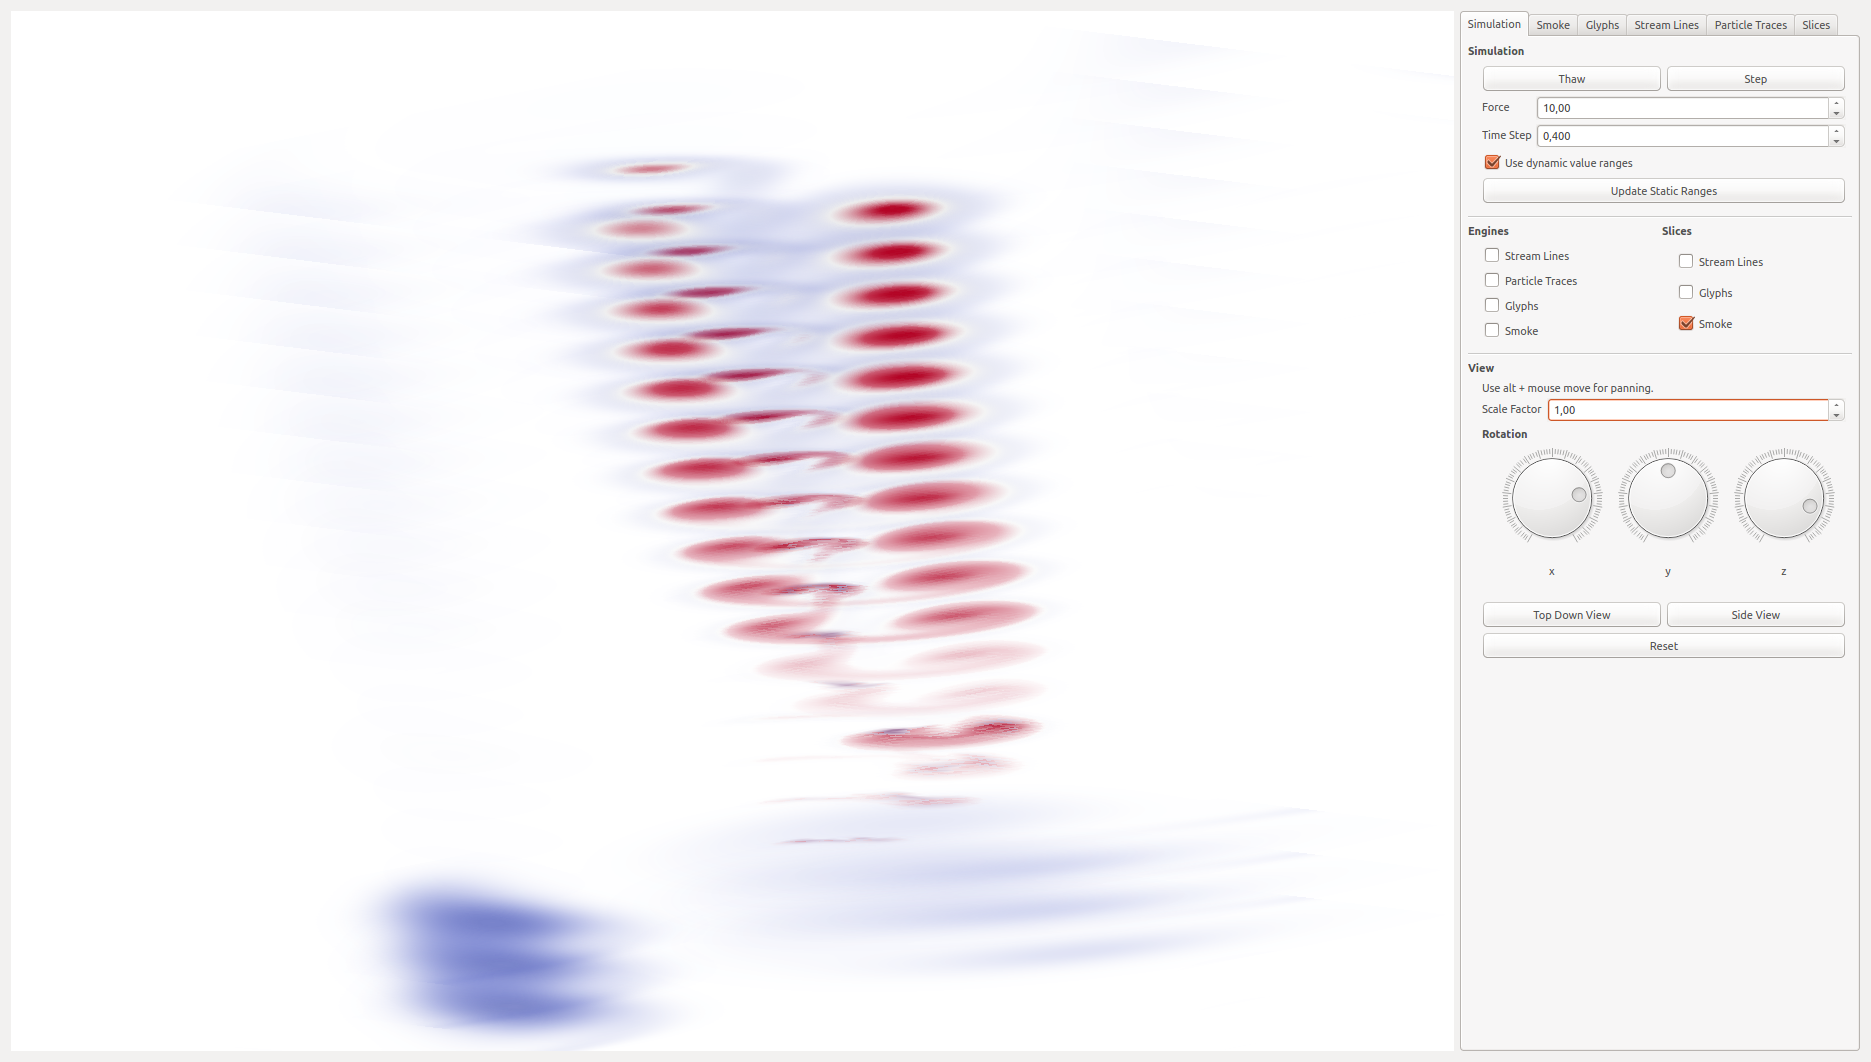
\includegraphics[width=0.9\textwidth, trim={35px 30px 430px 30px}, clip]{img/slices/diverging_sides}
		\caption{Slices showing fluid density using the divergent color map from a side view.}
		\label{fig:slices:colormap:side}
	\end{subfigure}
	\hspace{30px}
	\begin{subfigure}{0.45\textwidth}	
		\centering
		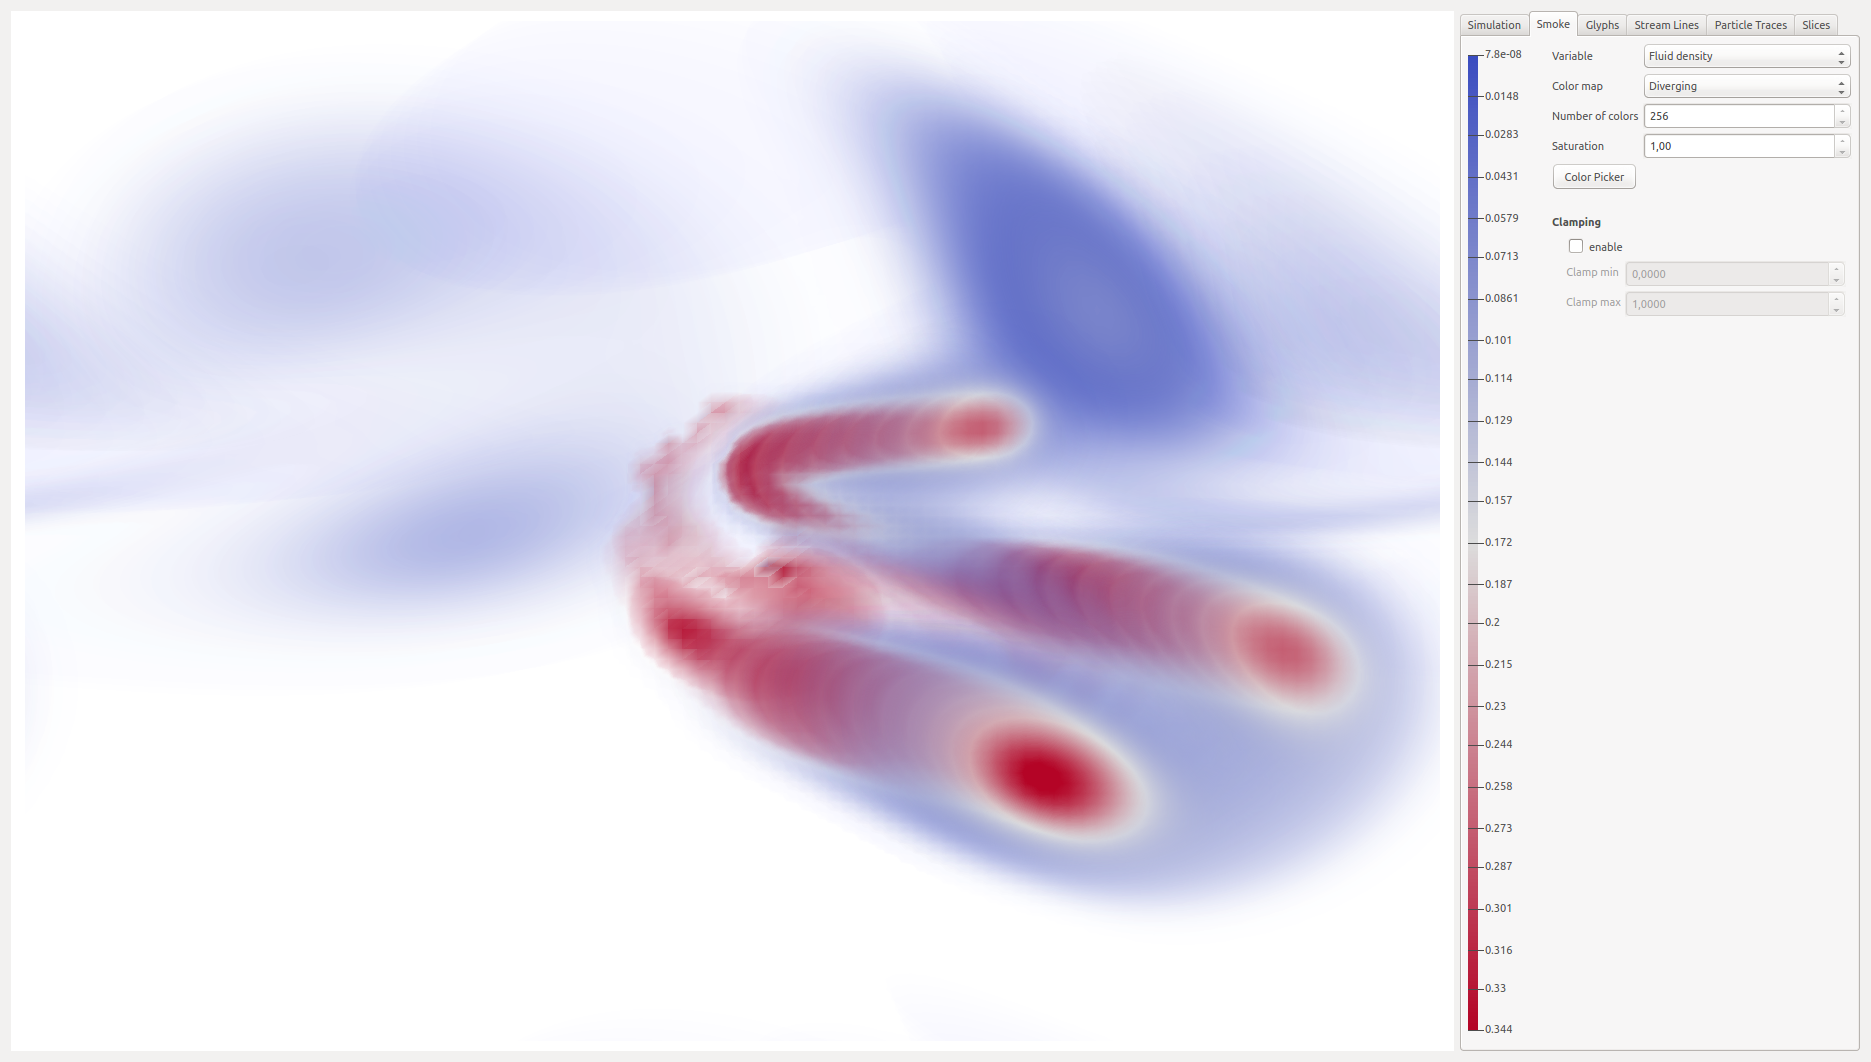
\includegraphics[width=0.9\textwidth, trim={35px 30px 430px 30px}, clip]{img/slices/divering}
		\caption{Slices showing fluid density using the divergent color map from top down view.}
		\label{fig:slices:colormap:top}
	\end{subfigure}
	\caption{Slices visualization combining 20 frames of a scalar color map visualization into a 3D visualization.}
	\label{fig:slices:colormap}
\end{figure}


\begin{figure}[tbh]
	\centering
	\begin{subfigure}{0.45\textwidth}
		\centering
		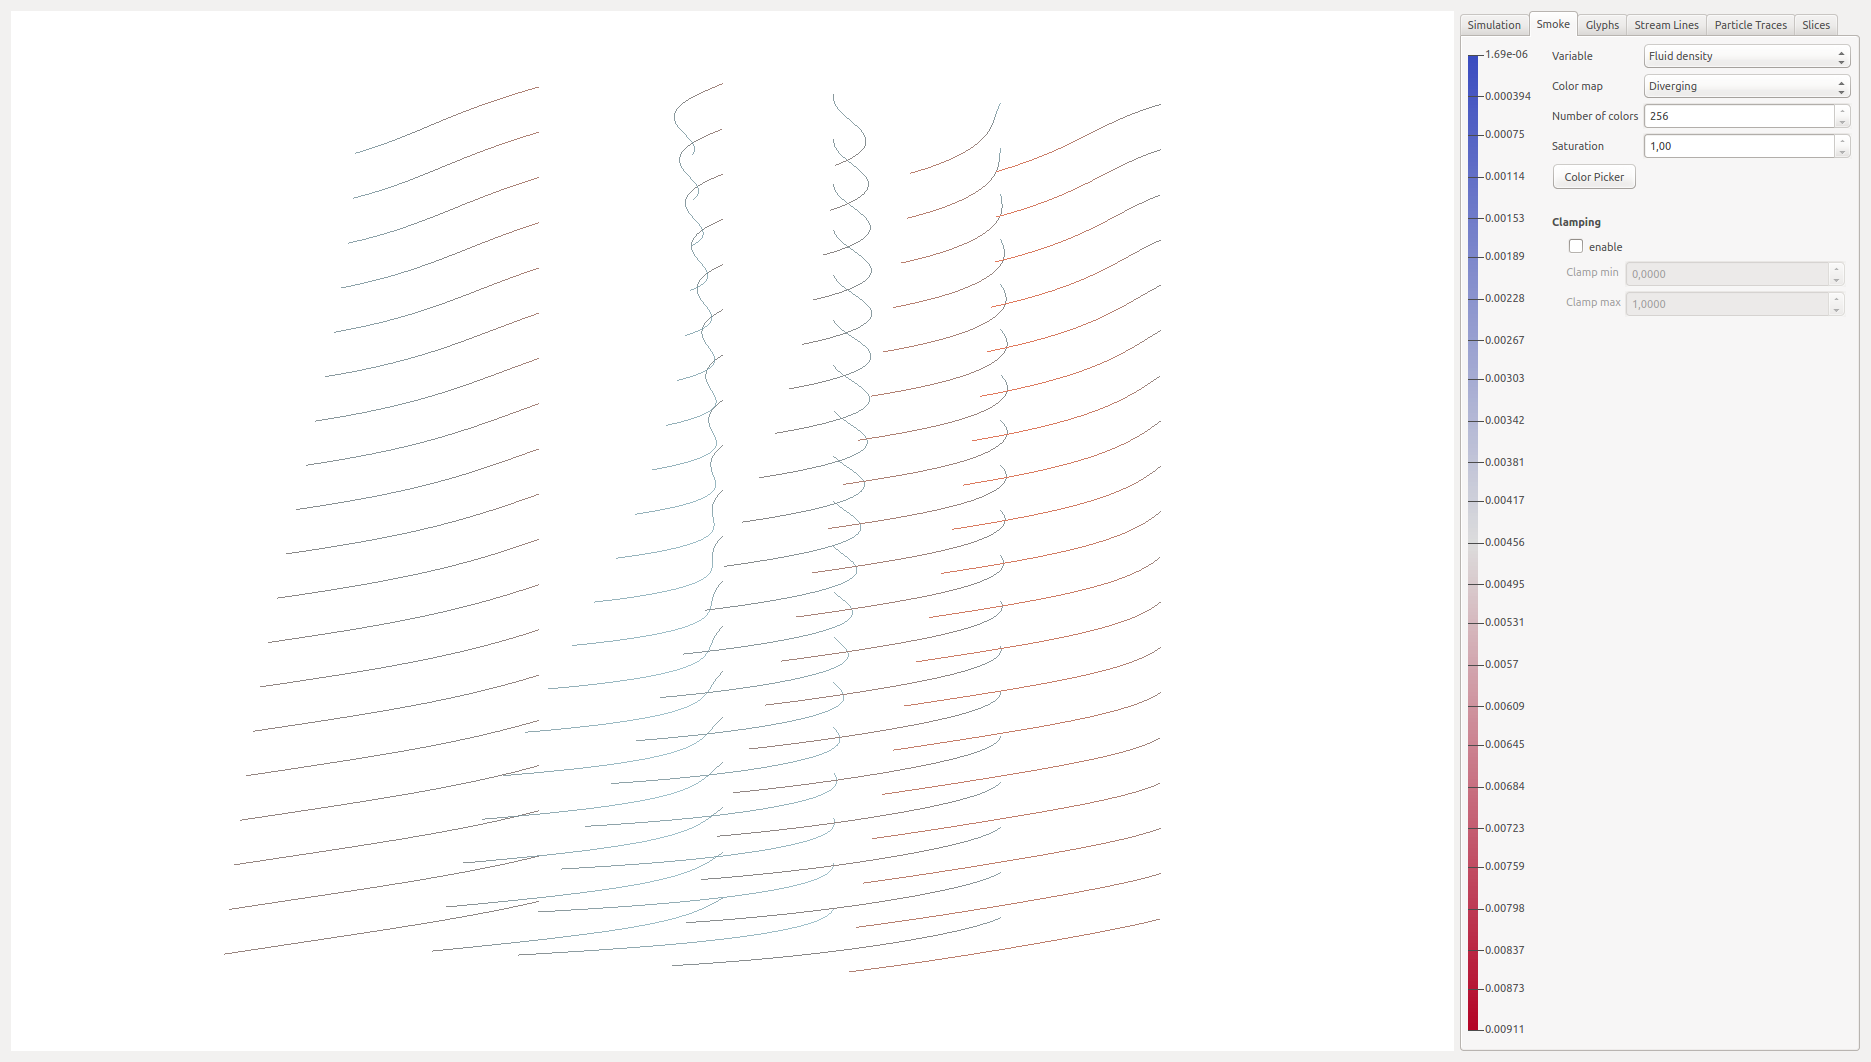
\includegraphics[width=0.9\textwidth, trim={35px 30px 430px 30px}, clip]{img/slices/streamlines_side}
		\caption{Slices showing the fluid density visualized using streamlines from a side view.}
		\label{fig:slices:streamlines:side}
	\end{subfigure}
	\hspace{30px}
	\begin{subfigure}{0.45\textwidth}	
		\centering
		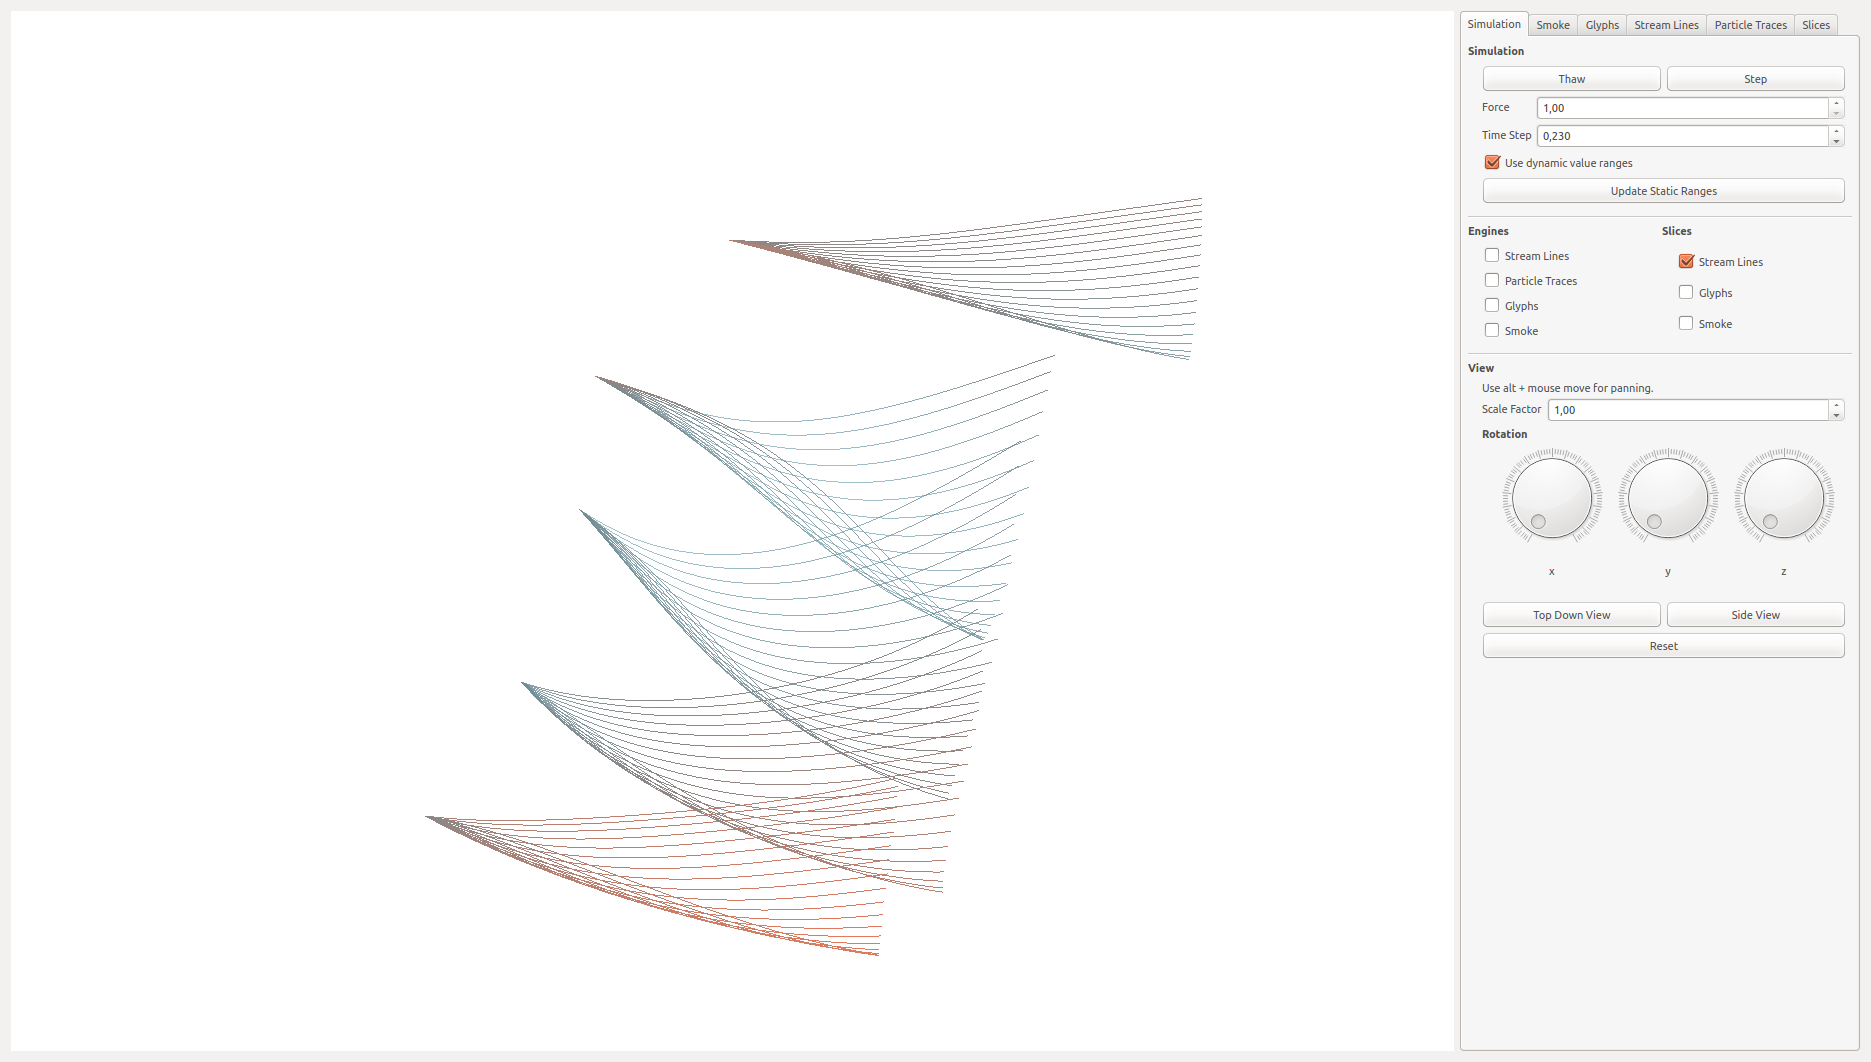
\includegraphics[width=0.9\textwidth, trim={35px 30px 430px 30px}, clip]{img/slices/streamlines_topdown}
		\caption{Slices showing the fluid density visualized using streamlines from a top down view.}
		\label{fig:slices:streamlines:top}
	\end{subfigure}
	\caption{Slices visualization combining 20 frames of streamlines visualization into a 3D visualization.}
	\label{fig:slices:streamlines}
\end{figure}




% section results (end)